\chapter{Implementation of spatial tournaments}
\label{chap:Three}
In this chapter we will discuss the source code committed to the
axelrod library to implement spatial topology. In addition, some
initial experiments and results will be discussed.

\section{Code Discussion}

As analyzed in \autoref{chap:Two}, the Axelrod library uses a
\texttt{Tournament()} class to run a round robin tournament. The
\texttt{RoundRobinTournament()} itself calls upon
another class the \texttt{Match Generator()} which is responsible to generate
the matches. In a round robin cause(\texttt{RoundRobinMatches()}), it generates
matches for each player
against the rest. The parameters and the index of the pair are push to it
by the \texttt{build single match()}. A generator that lives within the class.
For a round robin tournament the structure of the code is illustrated in~\ref{fig:rbr}.

\begin{figure}
\centering
    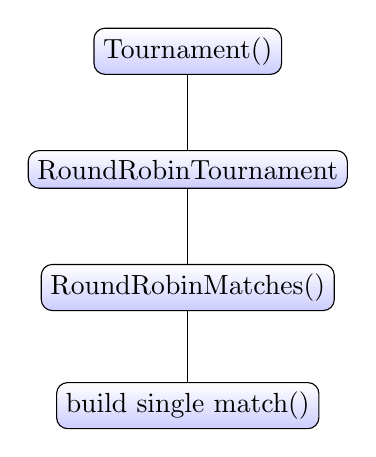
\begin{tikzpicture}[sibling distance=10em,
      every node/.style = {shape=rectangle, rounded corners,
        draw, align=center,
        top color=white, bottom color=blue!20}]]
      \node {Tournament()}
        child { node {RoundRobinTournament}
          child { node {RoundRobinMatches()}
            child { node {build single match()} } }
           };
    \end{tikzpicture}
  \caption{Code structure for a Round Robin tournament.}
  \label{fig:rbr}
\end{figure}

In order for us to implement a Spatial topology tournament we need to follow a
similar approach. Firstly a new \texttt{Match Generator()} class was written.
The \texttt{SpatialMatches()} is a class that generates spatially-structured
matches. In these matches, players interact only with their neighbors rather
than the entire population. According to \cite{Archdeacon1996} graphs can be
represents in many different ways, one of which is by lists of edges.
Due to a various number of python packages that are used for graph manipulation,
we want to generalize the representation of the edges.
For the \texttt{SpatialMatches()} do understand
which players are connected to each other, the edges are passed as a list
argument. The \texttt{SpatialMatches()} will only create matches between the
ending nodes of these edges. Finally the class \texttt{SpatialTournament()}
runs the spatial tournament. The code structure now that the spatial tournaments
have been added can be seen in Figure~\ref{fig:cds}

\begin{figure}
\centering
    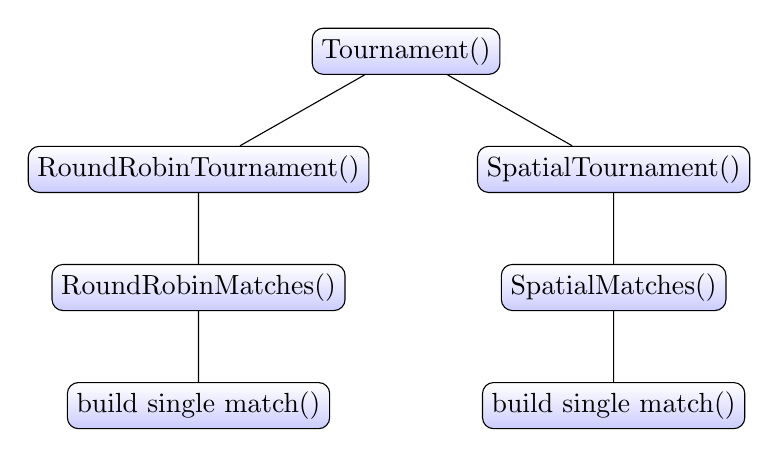
\begin{tikzpicture}[sibling distance=15em,
      every node/.style = {shape=rectangle, rounded corners,
        draw, align=center,
        top color=white, bottom color=blue!20}]]
      \node {Tournament()}
        child { node {RoundRobinTournament()}
          child { node {RoundRobinMatches()}
            child { node {build single match()} } }}
        child { node {SpatialTournament()}
          child { node {SpatialMatches()}
            child { node {build single match()} } }
           };
    \end{tikzpicture}
  \caption{Code structure for when Round Robin and Spatial tournaments are
           implemented.}
  \label{fig:cds}
\end{figure}

In Axelrod library all the components are automatically tested using a
combination of unit, property and integration tests(using \url{travis-ci.org}).
Once a new feature is added to the library, corresponding test must also be written.
The test are used to ensure compatibility and ensure that we get the expected
results. The tests for the \texttt{SpatialTournament()} can be found here :
\url{https://github.com/Axelrod-Python/Axelrod/blob/master/axelrod/tests/unit/test_tournament.py}
under the class \texttt{TestSpatialTournament()}.

In this section we gone through the structure of the source code for implementing
the Spatial Tournament, by adding to the Axelrod-Python library. Furthermore, now
that the code is usable in the following section we will go though some initial
analysis.

\section{First Experiment}

In this chapter we will be running some simple examples of spatial topology and
analyze the behavior of the strategies and the results. This will help us further
down to tackle the problem of how topology can affect the outcome of an IPD
competition and which strategies tend to perform well. Some of the most common
networks, based o literature, are a 2-D square lattice with four degrees
and a circle. Figure~\ref{fig:networks}, shows an example of these topologies.

\begin{figure}[h]
\centering
    \begin{subfigure}[t]{0.45\textwidth}
    \centering
        \includegraphics[width=\linewidth]{lattice_network.png}
    \caption{2-D square lattice network.}
    \end{subfigure}
\hfill
    \begin{subfigure}[t]{0.45\textwidth}\centering
    \centering
        \includegraphics[width=\linewidth]{circle_network.png}
    \caption{Circle network.}
    \end{subfigure}
\caption{Network topologies.}
\label{fig:networks}
\end{figure}

Thus, we will be performing our experiment with two different topologies, that
of a lattice and a circle. For each topology, 50 strategies out of the 132 of
Axelrod-Python library are chosen randomly. These 50 strategies create a
neighborhood. They are allocated on the graph, based on the topology, and they
compete with their neighbors on a IPD tournament. Once the first game is complete,
the strategies are randomly shuffled and allocated on the graph again.
They play another game of the IPD but this time with different
neighbors of they neighborhood. This is repeated 10 times and the random selection
of 50 players and creation of neighborhood is repeated 100 times.
Thus we achieve, 1000 tournaments with 100 different neighbors ,where each
neighborhood exists for 10 tournaments. Furthermore, each game of the IPD consists
of 200 turns and 10 repetitions.
By setting an axelrod-seed~\footnote{A function used by the library, which sets
both seeds for Numpy and the standard library.In general, seeds allow us
reproduce the same players and tournaments.}, the 100 neighborhoods for the topologies
are the same, of course their allocation to the graphs differs because of the
random shuffle.

\subsection{Circle Topology}
\label{sub:circle}

In the tournament with circle lattice while fifty players participated in each
of the hundred tournaments all 132 strategies of the Axelrod-Python library were
used at least once. Moreover, all strategies won, ranked 0, at least one
tournament. In Figure~\ref{fig:circle_winners}  we can see the number of times
each strategy has won a tournament in ascending order :

\begin{figure}[h!]
  \hspace*{-2cm}
    \includegraphics[scale=.15]{circle_winners.pdf}
    \caption{Number of winning tournaments by strategy in a circle topology.}
    \label{fig:circle_winners}
\end{figure}

As shown, %not clear at all, the figures are to large
the three strategies which achieved the most wins in the 1000 tournaments are :
Soft Joss: 0.9, Fortress3, Nice Average Copier. Soft Joss : 0.9, is an altered
version of Tit-For-Tat. The strategy emulates Tit-For-Tat but defects with a
probability of 0.9 when the opponent defects. Nice average copier will cooperate
with a probability p if the opponent's cooperation ratio is p. Starts by cooperating.
All three strategies achieved 14 wins. In a simple round robin tournament
all these have significant  different cooperating rating. Nice Average Copier,
is a cooperating strategy
where Soft Joss: 0.9 has an average cooperating rating and Fortress3 a low one.
We want to investigate any key factor for these strategies
achievement of first place even so in the original tournament the score quite
low.

The number that each strategy participated in the 1000 tournaments
is not clear. Thus, we can plot the number of participations of each strategy
as show in Figure ~\ref{fig:circle_freq}. It is shown that the range of participations varies
from 270 to 570 played tournaments and that Altenator played the most.
Furthermore, a more clear representation of the participations and strategies is
given by table in the Appendix. There is clear that the most common played
strategies were Altenator, ThueMorse, Shubik and Gradual. None of the first ranked
strategies.

\begin{figure}[h!]
\centering
    \includegraphics[scale=.12]{circle-frenquency.pdf}
    \caption{Number of participations in tournaments of each strategy.}
    \label{fig:circle_freq}
\end{figure}

Moreover, we can plot the number of participation against the number of times
the specific strategy has won to identify any correlation between these facts
Figure ~\ref{fig:circle_part-wins}. Though the strategies with the highest participation
ratio seem to have won tournaments, it is only a insignificant amount. strategies
with the highest number of wins see to have place an average number of tournaments.
By plotting the Frequency of the strategies against average score per turn,
we anticipated to have a positive correlation. As the more tournaments a strategy
competes in there is a higher probability that the strategy will be declared
the winner. Even so, from Figure~\ref{fig:circle_part-wins} we can assume that
they are is no significant correlation between these two facts.

\begin{figure}[h!]
\hspace*{-4cm}
    \begin{subfigure}[t]{1.4\textwidth}
    \centering
        \includegraphics[width=\linewidth]{circle-participated_wins.pdf}
    \caption{Number of participations against the number of winning tournaments.}
    \end{subfigure}
\hfill
\hspace*{-4cm}
    \begin{subfigure}[t]{1.4\textwidth}\centering
    \centering
        \includegraphics[width=\linewidth]{circle-freq-score.pdf}
    \caption{Frequency of strategies against winning tournaments.}
    \end{subfigure}
\caption{(a) Number of participations against the number of winning tournaments.
         (b) Frequency of strategies against winning tournaments.}
\label{fig:circle_part-wins}
\end{figure}

\newpage

Another factor we can investigate is the score of the neighborhood. Each strategy
belongs in a neighborhood of 50 strategies during the experiment. Plotting
the average score per turn against the neighbors overall average score. In
Figure~\ref{fig:circle-scatter-plot}, see an see as expected that each when the
higher the average score of the neighborhood the lowest the individuals score
per turn. Thus, a strategy in a neighborhood with winners is performing poorly.

\begin{figure}[h!]
\centering
    \includegraphics[scale=.12]{circle-scatter-plot.png}
    \caption{Scatter plot. Average score per turn and average neighborhood score.
             Circle topology.}
    \label{fig:circle-scatter-plot}
\end{figure}

Finally, a common methodology is building a regression model. We are building
a model wanting to identify any factor that can explain the average score of a
strategy. The model is the following :
\begin{equation}\label{regmodel}
average\_score = degree + average\_neighboorhood\_score + connectivity + frenquency
\end{equation}

and the output produced using python's statistic's tools is shown in Figure
~\ref{fig:circle-regression}. In the output we can see that Degree, average
neighborhood score and connectivity
are significant predictors with a p value less than an 0.00. However, the p-value
of frequency (0.446) is greater than the common alpha level of 0.05, which
indicates that frequency is not significant. We could foresee this from the undertaken
analysis. The coefficients of degree and connectivity point out the positivity
relationship of these variables and the average score. Average scores, again
something we could foresee, has a negative effect on the average score.
Additionally, an R square value of zero indicated that the model explains none of
the variability of the response data around its mean.

\begin{figure}[h!]
\centering
    \includegraphics[scale=.5]{circle-regression.png}
    \caption{Regression for circle topology results.}
    \label{fig:circle-regression}
\end{figure}
\newpage

\subsection{Lattice Topology}
\label{sub:lattice}

A similar approach as described above was taken for an experiment where
the tournaments had a lattice topology. The most frequented winner this time
was Adapative Pavlov 2006 (APavlov) with 15 wins ~\ref{fig:lattice-winners}.
Runner ups with 14 wins were Remorseful
Prober: 0.1, Fool Me Once and Inverse Punisher. APavlov is a strategy that attempts
to classify its opponent as one of five strategies: Cooperative, ALLD, STFT,
PavlovD, or Random. Then responds in a manner intended to achieve mutual
cooperation or to defect against uncooperative opponents.
None of this strategies ranked first in the circle topology. Furthermore, all
132 strategies participated at least on in this experiment and all achieved
first place at least once.

\begin{figure}[h!]
  \hspace*{-2cm}
    \includegraphics[scale=.15]{lattice-winners.pdf}
    \caption{Number of winning tournaments by strategy in a lattice topology.}
    \label{fig:lattice-winners}
\end{figure}

\newpage

An analysis to identify and factor for these results was performed.
The number of participations of each strategy, the ranks and average score
achieved by them were analyzed one again. Because the neighborhood are the same
for both topologies and what changes is only the degree, the plot for number of
participations should remain the same as shown in Figure~\ref{fig:circle_freq}.
Furthermore, the number of wins against number of participations are plot again
as well as the frequency against the winning tournaments. In the Participated
plot, a positive linear relation could exists but in the frequency plot
we can see no significant variation to the mean.

\newpage

\begin{figure}[h!]
\hspace*{-2cm}
    \begin{subfigure}[t]{1.2\textwidth}
    \centering
        \includegraphics[width=\linewidth]{lattice-participated_wins.pdf}
    \caption{Number of participations against the number of winning tournaments.}
    \end{subfigure}
\hfill
\hspace*{-2cm}
    \begin{subfigure}[t]{1.2\textwidth}\centering
    \centering
        \includegraphics[width=\linewidth]{lattice-freq-score.pdf}
    \caption{Frequency of strategies against winning tournaments.}
    \end{subfigure}
\caption{(a) Number of participations against the number of winning tournaments.
         (b) Frequency of strategies against winning tournaments. In a lattice
         topology.}
\label{fig:lattice-part-wins}
\end{figure}

\newpage

Moreover, a scatter plot to identify relationship with the average neighborhood
score is produced as well. Compared to our previous founding this plot shows a positive
correlation between the two factors~\ref{fig:lattice-scatter-plot}. Meaning, that you are more
likely to win
if you are in a winning neighborhood. This could be an affect of the topology.
More nodes interact with each other in a lattice and can create cluster more easy
than in circle topology.

\begin{figure}[h!]
\centering
    \includegraphics[scale=.12]{lattice-lines.png}
    \caption{Scatter plot. Average score per turn and average neighborhood score.
              Lattice topology}
    \label{fig:lattice-scatter-plot}
\end{figure}

To test our hypothesis we will again create a regression model, same as
in ~\ref{regmodel}. The results are shown here~\ref{fig:lattice-regression}.
Once more, degree, average neighborhood score and connectivity are significant
predictors with a p-value less than 0.00. Frequency, in the lattice topology
does not seem to have any effect either. What worth to point out is that
now all the significant predictors have a positive effect on the average score.
Finally, the R -square value indicates that only explains 3 \% of the variability
of the data around its mean.

\begin{figure}[h!]
\centering
    \includegraphics[scale=.5]{reg-lattice.png}
    \caption{Regression for circle topology results.}
    \label{fig:lattice-regression}
\end{figure}
\newpage

\subsection{Round Robin Tournament}
\label{sub:robin}

Once the experiment with the both topology was performed we wanted to compare
our results further and make an conclusion on the winning strategies. In order
to achieve that it was decided to run an experiment with the same 100 neighborhoods.
In time they strategies would compete on a round robin topology. Again the
number of turns was set to 200 but the repetitions to 100. All 132 strategies
compete at least once but only 72 of them achieved first place. In Figure
the results of this experiment are shown.

to be continuous ...

\subsection{Comparing Results}

In this section we will make a summary of all the previous analysis that was made
in~\ref{sub:circle, sub:lattice, sub:robin}. Furthermore, we will to compare
the winning strategies of each topology and identify any further relationship
between the performance of a strategy and the topology. From the analysis that
was performed in~\ref{sub:circle}, the winner came out to be 3 strategies that
performed the same, Soft Joss: 0.9, Fortress3, Nice Average Copier.
These strategies have not a similar characteristics like cooperating rating.
An attempt to find any significant reason as to why these strategies outperform
the rest return zero findings. Factors such as the connectivity of the graph,
the average score of the neighbors, the frequency that each strategy participated
and the degree of the graph had zero or non strongly significant effects.
In the circle topology the neighborhood score has a negative effect on the performance
of the strategy and the degree and connectivity of the graph a positive one.

Furthermore, the same approach was taken for~\ref{sub:lattice}. The winning
strategy of this experiment was announced to be Adapative Pavlov 2006, which
outperformed all the other strategies. Though the results as to why APavlov
did not differ much from the circle experiment. The were non strongly significant
factors identified from the analysis and the regression model. A difference
that was observed is that in the lattice example the average score of your
neighbors seem to have a positive effect on you. This is due to the structure of
the topology. The last experiment that was held was in~\ref{sub:robin}, where
the neighborhoods competed in an all out round robin tournament.

An illustration of the performance in all three topology for each strategy can
been seen in Figure.


In conclusion, the network topologies used in these examples seem to have be
simple and no real results were able to emerge. Moving forwards experiments
with more complicated and random topologies will be performed with all the 132
strategies of the Axelrod-Python library.
